%%========================================================================
%% LaTeX scriptiesjabloon
%%========================================================================


%%========================================================================
%% Preamble
%%========================================================================

\documentclass[pdftex,a4paper,12pt,twoside]{report}

%%---------- Extra functionaliteit ---------------------------------------

\usepackage[utf8]{inputenc}  % Accenten gebruiken in tekst (vb. é ipv \'e)
\usepackage{amsfonts}        % AMS math packages: extra wiskundige
\usepackage{amsmath}         %   symbolen (o.a. getallen-
\usepackage{amssymb}         %   verzamelingen N, R, Z, Q, etc.)
\usepackage[UKenglish]{babel}    % Taalinstellingen: woordsplitsingen,
                             %  commando's voor speciale karakters
                             %  ("dutch" voor NL)
							 %  ("UKenglish" voor brits engels)
\usepackage{eurosym}         % Euro-symbool €
\usepackage{graphicx}        % Invoegen van tekeningen
\usepackage[pdftex,bookmarks=true]{hyperref}
                             % PDF krijgt klikbare links & verwijzingen,
                             %  inhoudstafel
\usepackage{listings}        % Broncode mooi opmaken
\usepackage{multirow}        % Tekst over verschillende cellen in tabellen
\usepackage{rotating}        % Tabellen en figuren roteren
\usepackage{natbib}          % Betere bibliografiestijlen
\usepackage{fancyhdr}        % Pagina-opmaak met hoofd- en voettekst

%%---------- Layout ------------------------------------------------------

% hoofdingen, enz.
\pagestyle{fancy}

% lijn, wordt gebruikt in titelpagina
\newcommand{\HRule}{\rule{\linewidth}{0.5mm}}

% Leeg blad
\newcommand{\emptypage}{
\newpage
\thispagestyle{empty}
\mbox{}
\newpage
}
 
% Gebruik een schreefloos lettertype ipv het "oubollig" uitziende
% Computer Modern
\renewcommand{\familydefault}{\sfdefault}     

% Commando voor invoegen Java-broncodebestanden (dank aan Niels Corneille)
% Gebruik: \codefragment{source/MijnKlasse.java}{Uitleg bij de code}
\newcommand{\codefragment}[2]{ \lstset{%
  language=java,
  breaklines=true,
  float=th,
  caption={#2},
  basicstyle=\scriptsize,
  frame=single
}
\lstinputlisting{#1}}

%%---------- Documenteigenschappen ---------------------------------------
%% Vul dit aan met je eigen info:

% Je eigen naam
\newcommand{\studenta}{Pieter {Van Eeckhout}}

% Eventueel naam van een medestudent.
% Laat in commentaar indien niet van toepassing
%\newcommand{\studentb}{Steven Stevens}

% De naam van je stage-/bachelorproefbegeleider
\newcommand{\begeleider}{Johan {Van Schoor}} 

% De naam (én firma/organisatie) van je mentor/promotor
% Laat in commentaar indien niet van toepassing
%\newcommand{\mentor}{Jan Janssen, ACME Inc.}

% De titel van je scriptie/stageverslag
\newcommand{\titel}{Solving CAPTCHA using neural networks}

% Ondertitel
\newcommand{\ondertitel}{}

% Datum van indienen
\newcommand{\datum}{10 june 2013}

% Academiejaar
\newcommand{\academiejaar}{2012-2013}

%%========================================================================
%% Inhoud document
%%========================================================================

\begin{document}

%%---------- Front matter ------------------------------------------------
%% Het voorblad - Hier moet je in principe niets wijzigen.

\begin{titlepage}
\begin{center}

\includegraphics[width=4cm]{./img/FBO-NL.jpg}\\[.5cm]
% FBO-NL.jpg: 2000x1365 pixel, 300dpi, 16.93x11.56 cm, bb=0 0 480 328



Professional Bachelor in Applied Computer Science\\
Academic year \academiejaar

\vfill

\HRule \\[0.4cm]
{ \huge \bfseries \titel}\\[0.4cm]
\HRule \\[0.4cm]

{\Large \ondertitel}\\[0.4cm]

Submitted on \datum

\vfill

% Studenten en begeleiders
\begin{minipage}{0.49\textwidth}
\begin{flushleft}
\emph{Student\ifdefined\studentb en\fi :}\\
\studenta \\
\ifdefined\studentb \studentb \fi\par
\end{flushleft}
\end{minipage}
\begin{minipage}{0.49\textwidth}
\begin{flushright}
\emph{Mentor:}\\ \begeleider\\
\ifdefined\mentor \emph{Mentor:}\\ \mentor \fi
\end{flushright}
\end{minipage}

\end{center}

\end{titlepage}

% Schutblad

\emptypage

% Herhaling titelblad

\begin{titlepage}
\begin{center}
HoGent Business \& Information Management\\
Professional Bachelor in Applied Computer Science\\
Academic year \academiejaar

\vfill

\HRule \\[0.4cm]
{ \huge \bfseries \titel}\\[0.4cm]
\HRule \\[0.4cm]

{\Large \ondertitel}\\[0.4cm]

Submitted on \datum

\vfill

% Studenten en begeleiders
\begin{minipage}{0.49\textwidth}
\begin{flushleft}
\emph{Student\ifdefined\studentb en\fi :}\\
\studenta \\
\ifdefined\studentb \studentb \fi\par
\end{flushleft}
\end{minipage}
\begin{minipage}{0.49\textwidth}
\begin{flushright}
\emph{Mentor:}\\ \begeleider\\
\ifdefined\mentor \emph{Mentor:}\\ \mentor \fi
\end{flushright}
\end{minipage}

\end{center}

\end{titlepage}

%% Inhoudstafel

\tableofcontents

%%---------- Kern --------------------------------------------------------

\begin{abstract}

%% De "abstract" of samenvatting is een kernachtige (max 1 blz. voor een
% thesis) synthese van het document. In ons geval beschrijf je kort de
% probleemstelling en de context, de onderzoeksvragen, de aanpak en de
% resultaten. 

\end{abstract}

\chapter*{Preamble}
\label{ch:preamble}
Firstly, dear reader, I would like to thank you for taking the time to read this thesis. Without an audience this entire endeavour would not mean as much as it doe right now, while you are reading it's results. I personally believe this is because I would like my life not to go unnoticed. So if this thesis helps, or influences you in any way, the this work has gained more meaning.\\Secondly I would like to thank the following persons who have made it possible for me to arrive at this point. Special thanks and mentions go to:
\begin{itemize}
\item my parent, for giving me the opportunity and supplying the means for me to pursue my academic career.
\item my girlfriend, because she has helped me countless times. Because she helped through the rough spots. Because she never once complained about the time consuming job of writing this work.
\item my good friends, willing proof readers and content critics Wouter Dekens, Patrick Van Brussel and Thijs van der Burght.
\item Johan Van Schoor and Bert Van Vreckem for the support, organisation, guidance and feedback.
\end{itemize}
Bare in mind that this is not an exclusive list. So lastly I would like to thank all the other people who are not mentioned by name, like the teaching and support staff at University College Ghent.\\\\Ghent BELGIUM, June 2013
\begin{center}
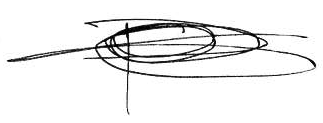
\includegraphics[width=5cm]{./img/signature.png}\\[.5cm]
\studenta
\end{center}
\chapter{Solving CAPTCHA using neural networks}
\label{ch:introduction}
\paragraph{The target audience.}
This thesis was written with an audience in mind that already has some technical understanding of computers and how they operate on hardware level (processor etc.). If you feel that your current knowledge is insufficient, or just want to read up some more, then I refer you to the ''How Computers Work - Processor and Main Memory'' \citep{Young2001} e-book.
\paragraph{The history of SPAM.} 
Ever since the internet has found its way into the daily usage in our society there have been people out there who don't always have other people's best interests in mind. In this particular case I am referring to people aiming to advertise their product, services, etc \ldots in an aggressive manner. The methods of advertising include but are not limited to: \begin{itemize}
\item Sending bulk emails without the recipients permission (SPAM). 
\item Posting irrelevant links and information on fora and various social media.
\item Flooding chat channels with their links and information. 
\end{itemize}
These emails, posts and messages inconvenience the end-users, requiring time to filter out the junk. The economic costs of SPAM has led to a decrease in the Japanese GDP by 500 billion Yen (3.78 billion Euro) in 2004 and were projected to reach a decrease of 1\% of the total GDP by 2010 unless adequate countermeasures were taken \citep{Ukai2007}. \citep{Khong2004} researched the economic arguments for regulating junk mails and the efficiency of these regulations.
\paragraph{Birth of CAPTCHA.} 
The two previously mentioned researches signify the importance and impact of SPAM on our daily lives. The users of the internet quickly tried to implement methods to prevent spammers from spreading their advertisements to the masses. Several prevention and detection methods and systems were developed successfully. These range from hidden text only visible to automated scripts, to invalid HTML tags. One of the methods developed for this purpose is a CAPTCHA test. CAPTCHA is an acronym based on the word ''capture'' and is spelled out completely as 'Completely Automated Public Turing test to tell Computers and Humans Apart'. An attempt to trademark  the term was made by Carnegie Mellon University on 15 October 2004, but the application was eventually dropped on 12 April 2008
\paragraph{Spammers fight back.}
All these prevention and detection methods did not stop the spammers from trying to reach an audience as large  as possible. They rely on this vast audience because of the return rates being as low as 0.0023\% \citep{Cobb2003}. Trying to reach such a large audience the spammers start to device ways to circumvent or break the existing systems. One of these methods is solving CAPTCHA tests making use of the adaptive learning and pattern recognizing capabilities of neural networks. These networks can be used to recognize letters from images with adversarial clutter.
This is the area I will focus on in this thesis. This thesis will list some of the difficulties regarding the extraction of relevant data from a CAPTCHA, and how to possibly overcome these difficulties. However the main focus will be on searching for the types and configuration of neural networks best used for pattern recognition.
\chapter{Premise and research questions}
\label{ch:Premise}

\section{Premise}
\label{sec:Premise}

%% VRAAGSTELLING
%% TODO: Write premise

\section{Research questions}
\label{sec:researquestions}

What different types of CAPTCHA exist?

What are the difficulties for solving a CAPTCHA automatically

What are the types of neural networks suitable for OCR

Is this a feasible endeavour at this point of personal computing power
%% TODO: Write research question

\chapter{Methodology}
\label{ch:methodology}



%% TODO: write methodology

\chapter{Corpus}
\label{ch:corpus}

%% TODO: define structure

\section{CAPTCHA}
\label{sec:captcha}

%% TODO: write methodology

\section{Neural Networks}
\label{sec:neuralnetworks}

%% TODO: write methodology

\section{Implementation}
\label{sec:implementation}

%% TODO: write methodology

%% 
%% Conclusie
%% 

\chapter{Conclusion}
\label{ch:conclusie}

%% TODO: write methodology

%%---------- Bijlagen ----------------------------------------------------

\appendix

\chapter{Sourcecode}
\label{ch:Sourcecode}

% Automatisch invoegen van al je Java broncode:
% 1/ maak een link naar je broncodedirectory naar subdirectory source
%      ln -s /path/to/java/src/ ./source
%    Of kopieer desnoods al je broncodebestanden. Zorg dat je
%    versiebeheersysteem deze directory negeert!
% 2/ Genereer source.tex met het script source.sh
%      ./source.sh
% 3/ Haal volgende regel uit commentaar
%% Java Broncode, gegenereerd door ./source.sh
% Waarschuwing: manuele wijzigingen worden overschreven!

\section{Package captchabuilder}

\section{Package captchacleanup}

\section{Package neuralnetworks}

\section{Package captchabuilder.builder}
\codefragment{source/captchabuilder/Captcha.java}{captchabuilder.Captcha}

\section{Package captchabuilder.elementcreator}

\section{Package captchabuilder.util}

\section{Package captchacleanup.image}

\section{Package captchacleanup.textfromimage}

\section{Package neuralnetworks.network}

\section{Package neuralnetworks.util}
\codefragment{source/captchabuilder/builder/BackgroundParser.java}{captchabuilder.builder.BackgroundParser}
\codefragment{source/captchabuilder/builder/BorderParser.java}{captchabuilder.builder.BorderParser}
\codefragment{source/captchabuilder/builder/CaptchaBuilder.java}{captchabuilder.builder.CaptchaBuilder}
\codefragment{source/captchabuilder/builder/CaptchaBuildSequenceParser.java}{captchabuilder.builder.CaptchaBuildSequenceParser}
\codefragment{source/captchabuilder/builder/ColorsParser.java}{captchabuilder.builder.ColorsParser}
\codefragment{source/captchabuilder/builder/GimpyParser.java}{captchabuilder.builder.GimpyParser}
\codefragment{source/captchabuilder/builder/NoiseParser.java}{captchabuilder.builder.NoiseParser}
\codefragment{source/captchabuilder/builder/TextParser.java}{captchabuilder.builder.TextParser}
\codefragment{source/captchabuilder/elementcreator/CaptchaElementCreatorBuilder.java}{captchabuilder.elementcreator.CaptchaElementCreatorBuilder}

\section{Package captchabuilder.elementcreator.producer}

\section{Package captchabuilder.elementcreator.renderer}
\codefragment{source/captchabuilder/util/ArrayUtil.java}{captchabuilder.util.ArrayUtil}
\codefragment{source/captchabuilder/util/CaptchaDAO.java}{captchabuilder.util.CaptchaDAO}
\codefragment{source/captchabuilder/util/ColorRangeRGBA.java}{captchabuilder.util.ColorRangeRGBA}

\section{Package captchabuilder.util.enums}
\codefragment{source/captchabuilder/util/ImageUtil.java}{captchabuilder.util.ImageUtil}
\codefragment{source/captchacleanup/image/ImageToArray.java}{captchacleanup.image.ImageToArray}
\codefragment{source/captchacleanup/image/ImageUtils.java}{captchacleanup.image.ImageUtils}
\codefragment{source/captchacleanup/textfromimage/GetImageText.java}{captchacleanup.textfromimage.GetImageText}
\codefragment{source/captchacleanup/textfromimage/TextRegion.java}{captchacleanup.textfromimage.TextRegion}

\section{Package neuralnetworks.network.encog}
\codefragment{source/neuralnetworks/network/NeuralNetworkActions.java}{neuralnetworks.network.NeuralNetworkActions}
\codefragment{source/neuralnetworks/network/NeuralNetwork.java}{neuralnetworks.network.NeuralNetwork}
\codefragment{source/neuralnetworks/util/CharacterPatternUtils.java}{neuralnetworks.util.CharacterPatternUtils}
\codefragment{source/neuralnetworks/util/EncogTrainingSet.java}{neuralnetworks.util.EncogTrainingSet}
\codefragment{source/neuralnetworks/util/ImageToInputPattern.java}{neuralnetworks.util.ImageToInputPattern}

\section{Package captchabuilder.elementcreator.producer.background}

\section{Package captchabuilder.elementcreator.producer.border}

\section{Package captchabuilder.elementcreator.producer.noise}

\section{Package captchabuilder.elementcreator.producer.text}

\section{Package captchabuilder.elementcreator.renderer.gimpy}

\section{Package captchabuilder.elementcreator.renderer.text}
\codefragment{source/captchabuilder/util/enums/CaptchaConstants.java}{captchabuilder.util.enums.CaptchaConstants}

\section{Package captchabuilder.util.enums.producer}

\section{Package captchabuilder.util.enums.renderer}
\codefragment{source/neuralnetworks/network/encog/EncogBasicNetworkBuilder.java}{neuralnetworks.network.encog.EncogBasicNetworkBuilder}
\codefragment{source/neuralnetworks/network/encog/EncogBasicNetwork.java}{neuralnetworks.network.encog.EncogBasicNetwork}
\codefragment{source/neuralnetworks/network/encog/EncogHopfieldNetworkBuilder.java}{neuralnetworks.network.encog.EncogHopfieldNetworkBuilder}
\codefragment{source/neuralnetworks/network/encog/EncogHopfieldNetwork.java}{neuralnetworks.network.encog.EncogHopfieldNetwork}

\section{Package neuralnetworks.network.encog.util}
\codefragment{source/captchabuilder/elementcreator/producer/background/AbstractBackgroundProducer.java}{captchabuilder.elementcreator.producer.background.AbstractBackgroundProducer}
\codefragment{source/captchabuilder/elementcreator/producer/background/BackgroundProducerBuilder.java}{captchabuilder.elementcreator.producer.background.BackgroundProducerBuilder}
\codefragment{source/captchabuilder/elementcreator/producer/background/BackgroundProducer.java}{captchabuilder.elementcreator.producer.background.BackgroundProducer}
\codefragment{source/captchabuilder/elementcreator/producer/background/FlatColorBackgroundProducer.java}{captchabuilder.elementcreator.producer.background.FlatColorBackgroundProducer}
\codefragment{source/captchabuilder/elementcreator/producer/background/SquigglesBackgroundProducer.java}{captchabuilder.elementcreator.producer.background.SquigglesBackgroundProducer}
\codefragment{source/captchabuilder/elementcreator/producer/background/TransparentBackgroundProducer.java}{captchabuilder.elementcreator.producer.background.TransparentBackgroundProducer}
\codefragment{source/captchabuilder/elementcreator/producer/background/TwoColorGradientBackgroundProducer.java}{captchabuilder.elementcreator.producer.background.TwoColorGradientBackgroundProducer}
\codefragment{source/captchabuilder/elementcreator/producer/border/AbstractBorderProducer.java}{captchabuilder.elementcreator.producer.border.AbstractBorderProducer}
\codefragment{source/captchabuilder/elementcreator/producer/border/BorderProducerBuilder.java}{captchabuilder.elementcreator.producer.border.BorderProducerBuilder}
\codefragment{source/captchabuilder/elementcreator/producer/border/BorderProducer.java}{captchabuilder.elementcreator.producer.border.BorderProducer}
\codefragment{source/captchabuilder/elementcreator/producer/border/SolidBorderProducer.java}{captchabuilder.elementcreator.producer.border.SolidBorderProducer}
\codefragment{source/captchabuilder/elementcreator/producer/noise/AbstractNoiseProducer.java}{captchabuilder.elementcreator.producer.noise.AbstractNoiseProducer}
\codefragment{source/captchabuilder/elementcreator/producer/noise/CurvedLineNoiseProducer.java}{captchabuilder.elementcreator.producer.noise.CurvedLineNoiseProducer}
\codefragment{source/captchabuilder/elementcreator/producer/noise/NoiseProducerBuilder.java}{captchabuilder.elementcreator.producer.noise.NoiseProducerBuilder}
\codefragment{source/captchabuilder/elementcreator/producer/noise/NoiseProducer.java}{captchabuilder.elementcreator.producer.noise.NoiseProducer}
\codefragment{source/captchabuilder/elementcreator/producer/noise/StraightLineNoiseProducer.java}{captchabuilder.elementcreator.producer.noise.StraightLineNoiseProducer}
\codefragment{source/captchabuilder/elementcreator/producer/text/AbstractTextProducer.java}{captchabuilder.elementcreator.producer.text.AbstractTextProducer}
\codefragment{source/captchabuilder/elementcreator/producer/text/AlphanumericTextProducer.java}{captchabuilder.elementcreator.producer.text.AlphanumericTextProducer}
\codefragment{source/captchabuilder/elementcreator/producer/text/ArabicTextProducer.java}{captchabuilder.elementcreator.producer.text.ArabicTextProducer}
\codefragment{source/captchabuilder/elementcreator/producer/text/ChineseTextProducer.java}{captchabuilder.elementcreator.producer.text.ChineseTextProducer}
\codefragment{source/captchabuilder/elementcreator/producer/text/LetterTextProducer.java}{captchabuilder.elementcreator.producer.text.LetterTextProducer}
\codefragment{source/captchabuilder/elementcreator/producer/text/NumbersProducer.java}{captchabuilder.elementcreator.producer.text.NumbersProducer}
\codefragment{source/captchabuilder/elementcreator/producer/text/ReducedAlphanumericTextProducer.java}{captchabuilder.elementcreator.producer.text.ReducedAlphanumericTextProducer}
\codefragment{source/captchabuilder/elementcreator/producer/text/SpecialAlphanumericTextProducer.java}{captchabuilder.elementcreator.producer.text.SpecialAlphanumericTextProducer}
\codefragment{source/captchabuilder/elementcreator/producer/text/SpecialLetterTextProducer.java}{captchabuilder.elementcreator.producer.text.SpecialLetterTextProducer}
\codefragment{source/captchabuilder/elementcreator/producer/text/SpecialNumbersProducer.java}{captchabuilder.elementcreator.producer.text.SpecialNumbersProducer}
\codefragment{source/captchabuilder/elementcreator/producer/text/TextProducerBuilder.java}{captchabuilder.elementcreator.producer.text.TextProducerBuilder}
\codefragment{source/captchabuilder/elementcreator/producer/text/TextProducer.java}{captchabuilder.elementcreator.producer.text.TextProducer}
\codefragment{source/captchabuilder/elementcreator/renderer/gimpy/AbstractGimpyRenderer.java}{captchabuilder.elementcreator.renderer.gimpy.AbstractGimpyRenderer}
\codefragment{source/captchabuilder/elementcreator/renderer/gimpy/BlockGimpyRenderer.java}{captchabuilder.elementcreator.renderer.gimpy.BlockGimpyRenderer}
\codefragment{source/captchabuilder/elementcreator/renderer/gimpy/DropShadowGimpyRenderer.java}{captchabuilder.elementcreator.renderer.gimpy.DropShadowGimpyRenderer}
\codefragment{source/captchabuilder/elementcreator/renderer/gimpy/FishEyeGimpyRenderer.java}{captchabuilder.elementcreator.renderer.gimpy.FishEyeGimpyRenderer}
\codefragment{source/captchabuilder/elementcreator/renderer/gimpy/GimpyRendererBuilder.java}{captchabuilder.elementcreator.renderer.gimpy.GimpyRendererBuilder}
\codefragment{source/captchabuilder/elementcreator/renderer/gimpy/GimpyRenderer.java}{captchabuilder.elementcreator.renderer.gimpy.GimpyRenderer}
\codefragment{source/captchabuilder/elementcreator/renderer/gimpy/RippleGimpyRenderer.java}{captchabuilder.elementcreator.renderer.gimpy.RippleGimpyRenderer}
\codefragment{source/captchabuilder/elementcreator/renderer/gimpy/ShearGimpyRenderer.java}{captchabuilder.elementcreator.renderer.gimpy.ShearGimpyRenderer}
\codefragment{source/captchabuilder/elementcreator/renderer/gimpy/StretchGimpyRenderer.java}{captchabuilder.elementcreator.renderer.gimpy.StretchGimpyRenderer}
\codefragment{source/captchabuilder/elementcreator/renderer/text/AbstractWordRenderer.java}{captchabuilder.elementcreator.renderer.text.AbstractWordRenderer}
\codefragment{source/captchabuilder/elementcreator/renderer/text/ColoredEdgesWordRenderer.java}{captchabuilder.elementcreator.renderer.text.ColoredEdgesWordRenderer}
\codefragment{source/captchabuilder/elementcreator/renderer/text/DefaultWordRenderer.java}{captchabuilder.elementcreator.renderer.text.DefaultWordRenderer}
\codefragment{source/captchabuilder/elementcreator/renderer/text/WordRendererBuilder.java}{captchabuilder.elementcreator.renderer.text.WordRendererBuilder}
\codefragment{source/captchabuilder/elementcreator/renderer/text/WordRenderer.java}{captchabuilder.elementcreator.renderer.text.WordRenderer}
\codefragment{source/captchabuilder/util/enums/producer/BackgroundProducerType.java}{captchabuilder.util.enums.producer.BackgroundProducerType}
\codefragment{source/captchabuilder/util/enums/producer/BorderProducerType.java}{captchabuilder.util.enums.producer.BorderProducerType}
\codefragment{source/captchabuilder/util/enums/producer/NoiseProducerType.java}{captchabuilder.util.enums.producer.NoiseProducerType}
\codefragment{source/captchabuilder/util/enums/producer/TextProducerType.java}{captchabuilder.util.enums.producer.TextProducerType}
\codefragment{source/captchabuilder/util/enums/renderer/GimpyRendererType.java}{captchabuilder.util.enums.renderer.GimpyRendererType}
\codefragment{source/captchabuilder/util/enums/renderer/WordRendererType.java}{captchabuilder.util.enums.renderer.WordRendererType}
\codefragment{source/neuralnetworks/network/encog/util/PropagationType.java}{neuralnetworks.network.encog.util.PropagationType}


\bibliographystyle{plainnat}
\bibliography{Solving_CAPTCHA_using_neural_networks}

%%---------- Back matter -------------------------------------------------

\listoffigures
\listoftables

% Lijst van broncode-listings. Kan je weglaten als je dit niet nodig hebt.
\lstlistoflistings

\end{document}